\documentclass[a4paper]{article}

\usepackage[per-mode=symbol,separate-uncertainty=true]{siunitx}
\usepackage{amsmath}
\usepackage{float}
\usepackage{graphicx}
\usepackage[a4paper,top=3cm,bottom=2cm,left=3cm,right=3cm,marginparwidth=1.75cm]{geometry}
\usepackage{mathtools}
\usepackage{siunitx}
\usepackage[colorlinks=true, allcolors=blue]{hyperref}

\sisetup{exponent-product=\cdot}

\title{Integrated System Architecture \\ Lab session 1 report}
\author{Marco Andorno (247222)\\ Michele Caon (253027) \\ Matteo Perotti (251453) \\ Giuseppe Sarda (xxxxxx)}

\begin{document}
\maketitle

\section{Filter design}
Following the rules given in the assignment, the main specifications were derived:
\begin{itemize}
    \item Filter type: IIR
    \item Filter order: \(N = 2\)
    \item Cutoff frequency: $f_c = \SI{2}{\kilo\hertz}$
    \item Sampling frequency: $f_s = \SI{10}{\kilo\hertz}$
    \item Data parallelism: $n_b = 12$
\end{itemize}
Then, using the provided example MATLAB script, the filter coefficients were found by means of the \texttt{butter} function. Real coefficients are then quantized as fixed point fractional number in the format $Q1.(n_b-1)$ ($Q1.11$ in our case) and expressed as integers on $n_b$ bits for the future C model and hardware filter. We will discover later that some care has to be taken when performing operations on the integer representation of fixed point numbers. 

Quantization is performed by truncation (\texttt{floor} function), so that the maximum error is equal to:
\[\varepsilon_{max} = 2^{-(n_b-1)} = 2^{-11} = 0.049\%\]
We accept that this error could be reduced by rounding and that truncation introduces a negative bias by approximating always towards \(-\infty\), because on the other hand truncation is much easier to implement in hardware, where it just represent an arithmetic shift.

The resulting difference equation is in the end:
\[y[n] = b_0x[n] + b_1x[n-1] + b_2x[n-2] - a_1y[n-1] - a_2y[n-2]\]
where
\begin{description}
    \item \(b_0 = 0.20654 = 423\)
    \item \(b_1 = 0.41309 = 846\)
    \item \(b_2 = 0.20654 = 423\)
    \item \(a_1 = -0.36963 = -757\)
    \item \(a_2 = 0.19580 = 401\)
\end{description}

\begin{figure}[hbtp]
    \centering
    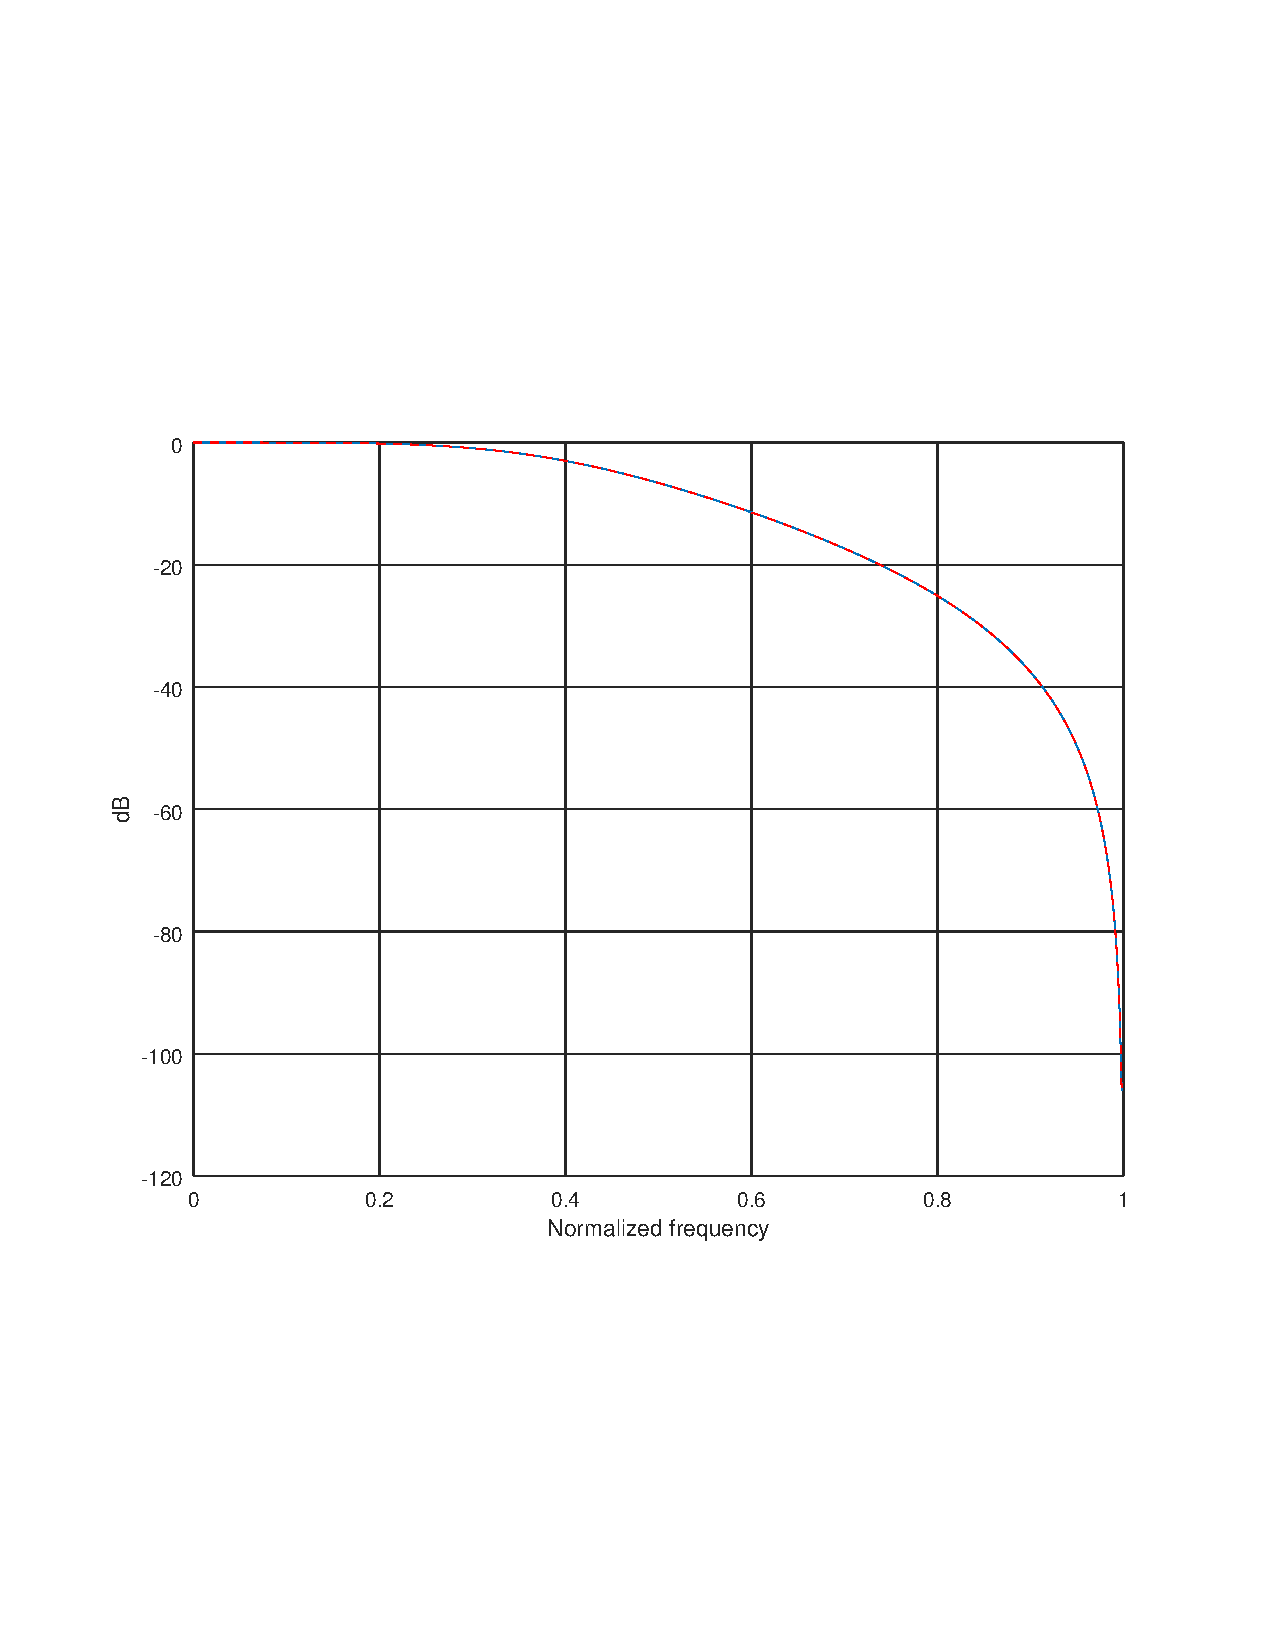
\includegraphics[width=.8\linewidth]{media/tf.pdf}
    \caption{Bode plot of the filter frequency response}
    \label{fig:tf}
\end{figure}
Figure~\ref{fig:tf} shows the transfer function of the filter computed from both the original coefficients and the quantized ones. The two curves cannot be told apart because the error is too small (\num{5.42e-7} in the worst case).

\begin{figure}[hbtp]
    \centering
    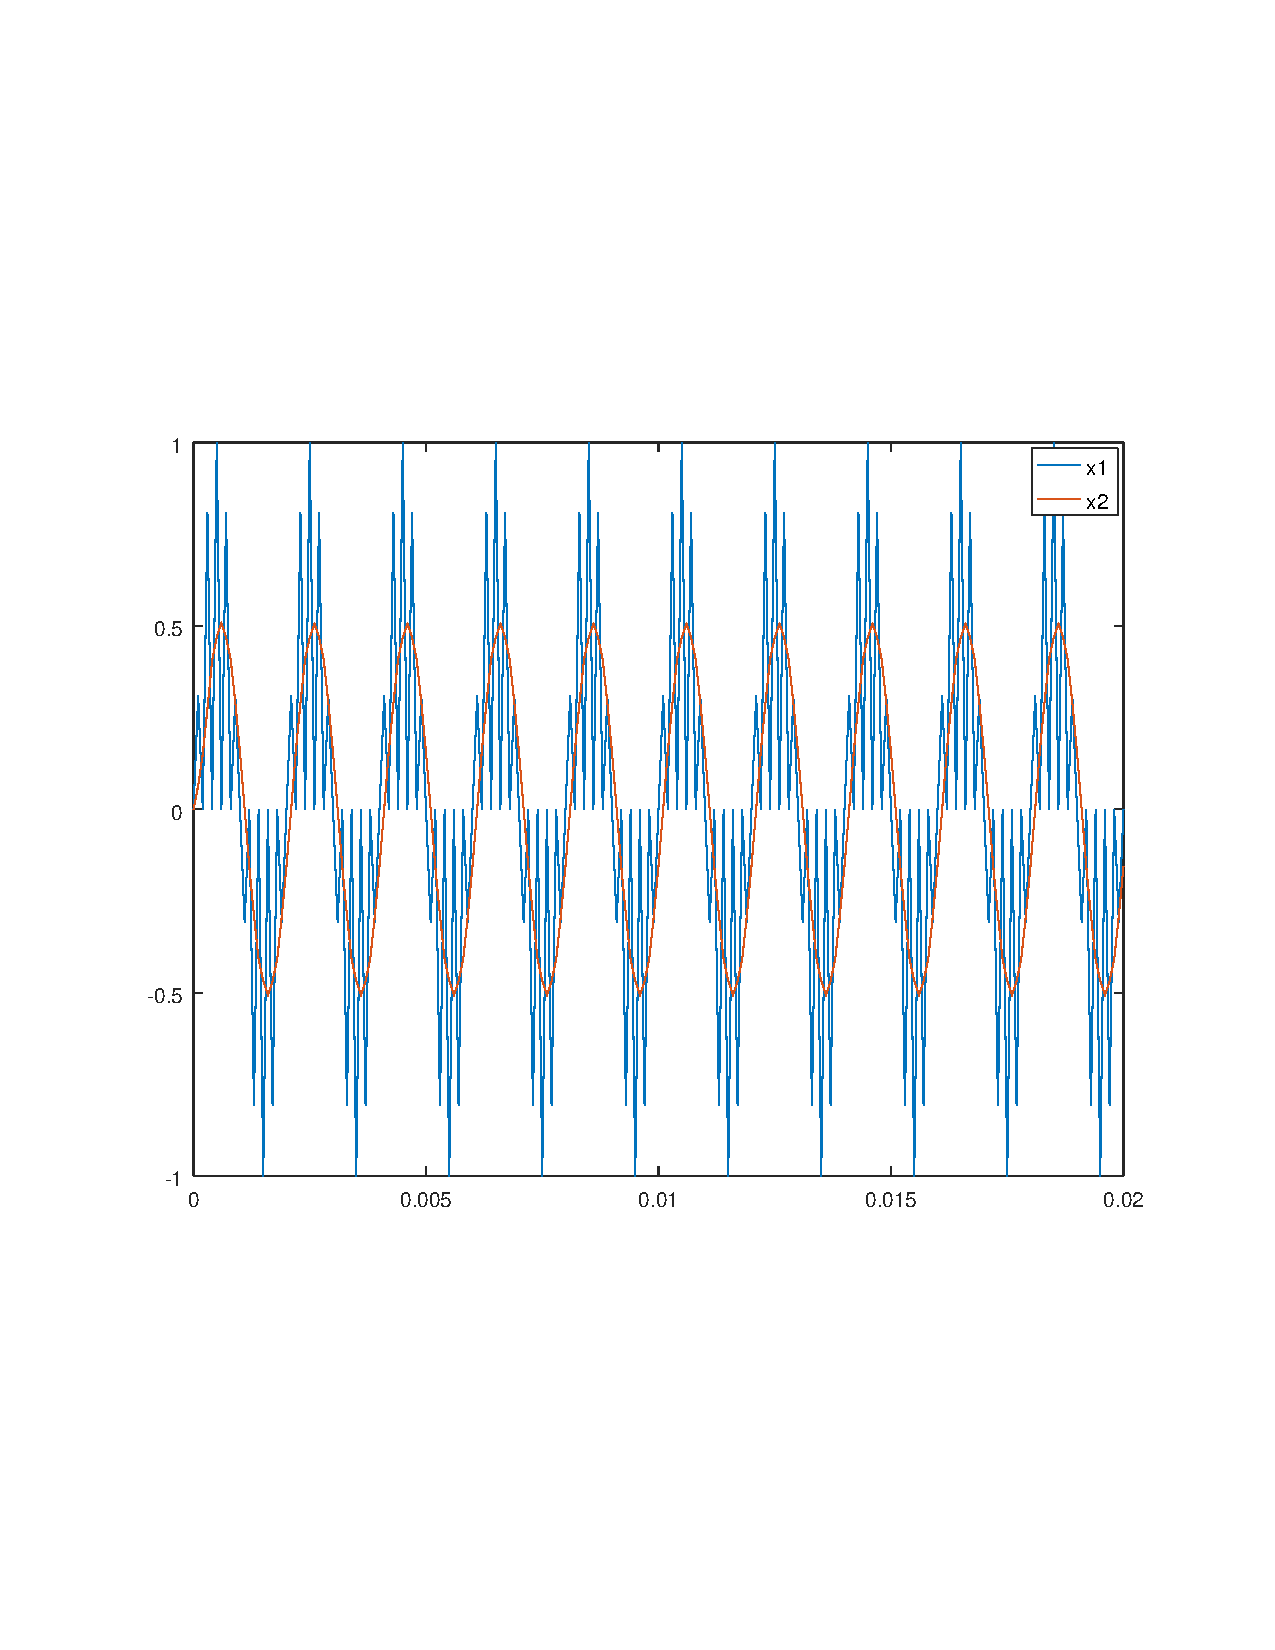
\includegraphics[width=\linewidth]{media/sine.pdf}
    \caption{Input and output waveforms}
    \label{fig:sine}
\end{figure}
Figure~\ref{fig:sine} on the other hand shows the time domain waveforms of an input signal $x_1(t)$, in blue, containing two frequency components one in band and one out of band, and the corresponding output $x_2(t)$, in red, where only the in-band component survives.

\end{document}

